\chapter{Results}

We found all signed snarks up to 18 vertices.

\begin{figure}[h]
    \centering
    \begin{tabular}{ |c|c|c|c|c| }
        \hline
        N & G & non-equivalent signatures per G & signed G & signed snarks \\
        \hline
        \hline
        4 & 1 & 8 & 8 & 0 \\
        \hline
        6 & 2 & 16 & 32 & 0 \\
        \hline
        8 & 5 & 32 & 160 & 1 \\
        \hline
        10 & 19 & 64 & 1216 & 48 \\
        \hline
        12 & 85 & 128 & 10 880 & 227 \\
        \hline
        14 & 509 & 256 & 130 304 & 2768 \\
        \hline
        16 & 4060 & 512 & 2 078 720 & 31 869 \\
        \hline
        18 & 41 301 & 1024 & 42 292 224 & 437 381 \\
        \hline
        %20 & 510 489 & 2048 & 1 045 481 472 & ? \\
        %\hline
    \end{tabular}
    \caption[Basic signed graph data]{Basic signed graph data. Here signed snarks were not yet filtered for isomorphisms.}
\end{figure}

The smallest signed snark is smaller than the Petersen graph (smallest snark), it is the projection of a 3D cube.

\begin{figure}[h]
    \centering
    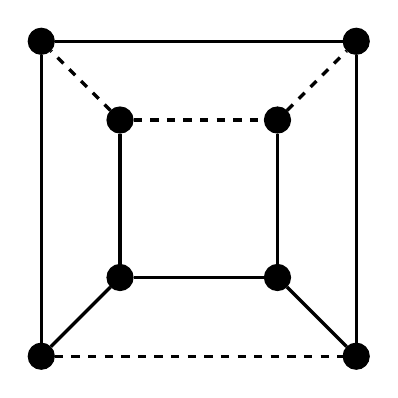
\begin{tikzpicture}
        \begin{scope}[every node/.style={circle,draw,fill=black}]
            \node (1) at (-1, -1) {};
            \node (2) at (-1, 1) {};
            \node (3) at (1, -1) {};
            \node (4) at (1, 1) {};
            \node (5) at (-2, -2) {};
            \node (6) at (-2, 2) {};
            \node (7) at (2, -2) {};
            \node (8) at (2, 2) {};
        \end{scope}
        \begin{scope}[every edge/.style={draw,very thick}]
            \path
                (1) edge (2)
                (1) edge (3)
                (1) edge (5)
                (2) edge [dashed] (4)
                (2) edge [dashed] (6)
                (3) edge (4)
                (3) edge (7)
                (4) edge [dashed] (8)
                (5) edge (6)
                (5) edge [dashed] (7)
                (6) edge (8)
                (7) edge (8);
        \end{scope}
    \end{tikzpicture}
    \caption{Smallest snark}
\end{figure}

Similarly to regular snarks, there are trivial properties of signed graphs that don't allow the possibility of a 3-edge-coloring. The following unsigned graph is the smallest graph that doesn't have a 3-edge-colorable signature.

\begin{figure}[h]\label{smallest-uncolorable}
    \centering
    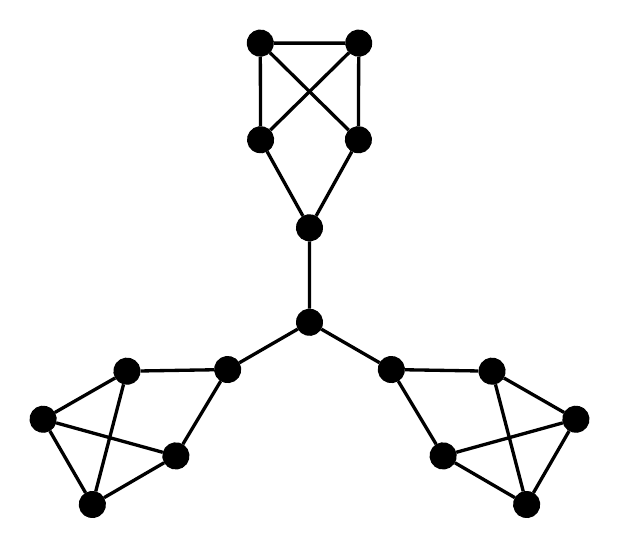
\begin{tikzpicture}[scale=0.6]
        \begin{scope}[every node/.style={circle,draw,fill=black,rotate=30}]
            \node (1) at (0,0) {};
            \node (2) at (xyz polar cs:angle=90, radius=2) {};
            \node (3) at (xyz polar cs:angle=210, radius=2) {};
            \node (4) at (xyz polar cs:angle=330, radius=2) {};
            \node (5) at (xyz polar cs:angle=75, radius=4) {};
            \node (6) at (xyz polar cs:angle=80, radius=6) {};
            \node (7) at (xyz polar cs:angle=100, radius=6) {};
            \node (8) at (xyz polar cs:angle=105, radius=4) {};
            \node (9) at (xyz polar cs:angle=195, radius=4) {};
            \node (10) at (xyz polar cs:angle=200, radius=6) {};
            \node (11) at (xyz polar cs:angle=220, radius=6) {};
            \node (12) at (xyz polar cs:angle=225, radius=4) {};
            \node (13) at (xyz polar cs:angle=315, radius=4) {};
            \node (14) at (xyz polar cs:angle=320, radius=6) {};
            \node (15) at (xyz polar cs:angle=340, radius=6) {};
            \node (16) at (xyz polar cs:angle=345, radius=4) {};
        \end{scope}
        \begin{scope}[every edge/.style={draw,very thick}]
            \path
                (1) edge (2)
                (2) edge (5)
                (2) edge (8)
                (5) edge (6)
                (5) edge (7)
                (6) edge (8)
                (6) edge (7)
                (7) edge (8);
            \path
                (1) edge (3)
                (3) edge (9)
                (3) edge (12)
                (9) edge (10)
                (9) edge (11)
                (10) edge (12)
                (10) edge (11)
                (11) edge (12);
            \path
                (1) edge (4)
                (4) edge (13)
                (4) edge (16)
                (13) edge (14)
                (13) edge (15)
                (14) edge (16)
                (14) edge (15)
                (15) edge (16);
        \end{scope}
    \end{tikzpicture}
    \hspace{0.1\textwidth}
    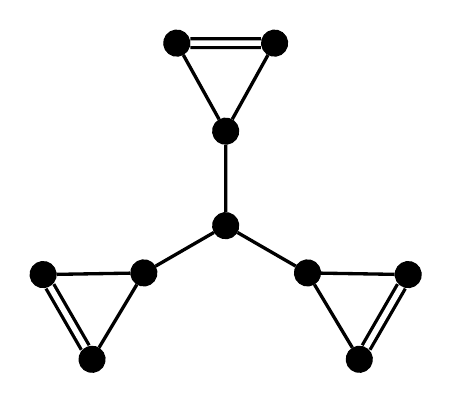
\begin{tikzpicture}[scale=0.6]
        \begin{scope}[every node/.style={circle,draw,fill=black,rotate=30}]
            \node (1) at (0,0) {};
            \node (2) at (xyz polar cs:angle=90, radius=2) {};
            \node (3) at (xyz polar cs:angle=210, radius=2) {};
            \node (4) at (xyz polar cs:angle=330, radius=2) {};
            \node (5) at (xyz polar cs:angle=75, radius=4) {};
            \node (8) at (xyz polar cs:angle=105, radius=4) {};
            \node (9) at (xyz polar cs:angle=195, radius=4) {};
            \node (12) at (xyz polar cs:angle=225, radius=4) {};
            \node (13) at (xyz polar cs:angle=315, radius=4) {};
            \node (16) at (xyz polar cs:angle=345, radius=4) {};
        \end{scope}
        \begin{scope}[every edge/.style={draw,very thick}]
            \path
                (1) edge (2)
                (2) edge (5)
                (2) edge (8);
            \path
                (1) edge (3)
                (3) edge (9)
                (3) edge (12);
            \path
                (1) edge (4)
                (4) edge (13)
                (4) edge (16);
        \end{scope}
        \begin{scope}[every edge/.style={draw, very thick, double distance=2pt}]
            \path
                (5) edge (8)
                (9) edge (12)
                (13) edge (16);
        \end{scope}
    \end{tikzpicture}

    \caption[Smallest simple graph without a 3-edge-colorable signature]{Smallest simple graph without a 3-edge-colorable signature and a simplified version allowing duplicate edges.}
\end{figure}

\begin{theorem}
    An unsigned graph $G$ has a signature that admits a 3-edge-coloring if and only if it has a 1-factor (1-regular subgraph with the same vertex set).
\end{theorem}

\textit{Proof.} If there is a signature and a 3-edge-coloring on it, the edges colored $0$ form by the definition of a proper edge coloring a perfect matching. Now let $M \subseteq E(G)$ be a 1-factor. Let's assign the color $0$ to these edges again and remove them from $G$. After removing a 1-factor from a cubic graph we obtain a 2-factor, a set of disjunct cycles (if two cycles would have a common vertex, its degree in the original graph would have to be at least 4). According to \Cref{th:brooks} for the cycles to be colorable, we assign any balanced signature to even cycles and any unbalanced signature to odd cycles. All cycles from this 2-factor will now be 2-edge-colorable with colors $1$ and $-1$ and combined with the $0$-colored 1-factor we obtain a 3-edge-colorable signed cubic graph. \qed

The graph in \Cref{smallest-uncolorable} has no 1-factor. (The middle vertex has to be connected to one of the three triangles and the other two triangles will not have a matching.)
